\begin{document}

\def\title{CSM test}

\newcommand{\qitem}{\qpart\item}
\newcommand{\test}{../../testing}

\renewcommand{\labelenumi}{(\alph{enumi})} % change default enum format to (a)
\renewcommand{\theenumi}{(\alph{enumi})} % fix reference format accordingly.
\renewcommand{\labelenumii}{\roman{enumii}.} % second level labels.
\renewcommand{\theenumii}{\roman{enumii}.}

\maketitle

\vspace{0.5em}

\begin{qunlist}

% % {\Large \textbf{Mechanical:}}
\qns{First-Order Differential Equation Practice}
\qcontributor{Elena Jia}

\begin{enumerate}

\qitem Solve the equation $\frac{d}{dt} f(t) = 7 f(t) $ given that $f(0) = 3$

\sol{
	This is a basic first-order differential eqution practice. We know the solution of the equation $\frac{d}{dt} f(t) = 7 f(t)$ is in the form $f(t) = A e^{7t}$, as we can check by plugging it into the differential equation. We can find the value of $A$ by using $f(0) = 3$. The final solution is $f(t) = 3 e^{7t}$.
}

\qitem Solve the equation $\frac{d}{dt} f(t) + 5 f(t) = 0 $ given that $f(0) = 2$

\sol{
	$f(t) = 2 e^{-5t}$.
}

\qitem Solve the equation $3 \frac{d}{dt} f(t) + 6 f(t) = 0$ given that $f(0) = 7$

\sol{
	$f(t) = 7 e^{-2t}$.
}

\qitem Solve the equation $\frac{d}{dt} f(t) = 2f(t) + 2 $ given that $f(0) = 3$

\sol{
	To get started on this problem,  we can write the equation as $\frac{d}{dt} f(t) + 1 = 2(f(t) + 1) $. Then we solve for $f(t)+1$ like the previous problems and obtain $f(t)+1 = 4 e^{2t}$. The final solution is $f(t) = 4 e^{2t} - 1$.
}


\qitem Solve the equation $5\frac{d}{dt} f(t) + 3f(t) - 10 = 0 $ given that $f(0) = 8$

\sol{
	$f(t) = \frac{14}{3}e^{\frac{-3}{5} t} + \frac{10}{3}$.
}



\qitem Solve the equation $6\frac{d}{dt} f(t) + 4 = 3f(t) $ given that $f(0) = \frac{1}{3}$

\sol{
	$f(t) = - e^{\frac{1}{2} t} + \frac{4}{3} $.
}


\qitem Solve the equation $3f(t) - 6 f'(t) = 4$ given that $f(2) = \frac{1}{3}$

\sol{
	$f(t) = -e^{\frac{1}{2} t - 1} + \frac{4}{3}$ \\
}

% \qitem  Solve the equation $f'(t) = 5f(t) + 8 e^{5t}$ given that $f(0) = 7$

% \sol{
% 	$7e^{5t}+8e^{5t}t$.
% }


% \qitem  Solve the equation $f'(t) = af(t) + k e^{bt}$

% \sol{
% 	$ce^{at}-\frac{ke^{bt}}{a-b}$.
% }



\end{enumerate}
% \begin{figure}[H]
	\begin{centering}
		\begin{circuitikz}
			\draw (0, 4)
			to[V =$V_s$] (0, 0);
			\draw (0, 4)
			to[switch,l^=\mbox{$t = 0$}](4,4)
			(4,4) to[R = $R$,v=$V_R(t)$,i>^=$i_R(t)$] (7,4)	
			to [short] (9,4)
			to[C = $C$, v=$V_C(t)$,i>^=$i_C(t)$] (9,0)
			to [short] (0,0);
		\end{circuitikz}
		\caption{\label{fig:circuit}RC Circuit with Voltage Source}
	\end{centering}
\end{figure}

% \qns{Fun with Inductors}
\qcontributor{Arda Sahiner}

\begin{enumerate}

\begin{figure}[H]
 \centering
 \begin{circuitikz}
	\draw
	(0, 0)
	to[V=$V_{in}$] ++ (0, -4)
	to[short, -o] ++(6, 0)

	(0, 0)
	to[L, l=$L$, i=$I_L$] ++ (3, 0)
	to[short] ++(2, 0)

	(3, 0)
	to[opening switch,l^=\mbox{$t = 0$}] ++(0, -2)
	to[R, l=$R_1$] ++(0, -2)

	(5, 0)
	to[switch, l^=\mbox{$t = 0$}] ++(0, -2)
	to[R, l=$R_2$] ++ (0, -2)

	(5, -2)
	to[short, -o] ++(1, 0)
	to[open, v^=$V_{out}$] ++(0, -2)

	(3, -1) node[left]{$S_1$}
	(5, -1) node[left]{$S_2$}
	;
\end{circuitikz}
 \caption{Circuit A}
\end{figure}

\qitem Consider circuit A. Assuming that for $t<0$, switch $S_1$ is on and switch $S_2$ is off (and both switches have been in these states indefinitely), what is $i_L(0)$?

\sol{
When $S_1$ is on and $S_2$ is off for a long period of time, $\frac{di_L}{dt} = 0$ because the circuit will have reached a steady state, and the current through $R_1$ will be equal to $i_L$. We find
$$V_{in} - V_L - V_{R_1} = 0$$
$$V_{in} - L\frac{di_L}{dt}(0) - i_L(0)R_1 = 0$$
$$V_{in} - i_L(0)R_1 = 0$$
$$i_L(0) = \frac{V_{in}}{R_1}$$
}

\qitem Now let's assume that for $t \geq 0$, $S_1$ is off and $S_2$ is on. Solve for $V_{out}(t)$ for $t \geq 0$.

\sol {
$$V_{in} - V_L - V_{out} = 0$$
$$V_{in} - L\frac{di_L}{dt} - i_LR_2 = 0$$
$$\frac{di_L}{dt} + \frac{R_2}{L}i_L = \frac{V_{in}}{L}$$

This is a non-homogenous first order differential equation in $i_L$. We can solve for $i_L(t)$ and then use Ohm's law to find $V_{out}(t)$ after this has been solved.
$$\frac{di_L}{dt} + \frac{R_2}{L}(i_L - \frac{V_{in}}{R_2}) = 0$$
Let $\tilde{i_L} = i_L - \frac{V_{in}}{R_2}$. We now have:
$$\frac{d\tilde{i}_L}{dt} + \frac{R_2}{L}\tilde{i}_L = 0$$

The general solution is given by:
$$\tilde{i}_L(t) = c_1 e^{-\frac{R_2}{L}t}$$
Resubstituting back $i_L$, we have:
$$i_L(t) = \frac{V_{in}}{R_2} + c_1 e^{-\frac{R_2}{L}t}$$

Applying initial conditions, we know:
$$i_L(0) = \frac{V_{in}}{R_2} + c_1 = \frac{V_{in}}{R_1}$$
$$c_1 = \frac{V_{in}}{R_1} - \frac{V_{in}}{R_2}$$

Our solution for $i_L(t)$ thus becomes:
$$i_L(t) = \frac{V_{in}}{R_2} + (\frac{V_{in}}{R_1} - \frac{V_{in}}{R_2})e^{-\frac{R_2}{L}t}$$
Since $V_{out}(t) = i_L(t)R_2$, 
$$V_{out}(t) = V_{in}(1 + (\frac{R_2}{R_1} - 1)e^{-\frac{R_2}{L}t})$$
}

\qitem If $V_{in} = 1 V$, $L = 1 nH$, $R_1 = 1 k\Omega$, and $R_2 =10 k\Omega$, what is the maximum value of $V_{out}(t)$ for $t \geq 0$?

\sol{
Since the coefficient in front of our time-varying component $e^{-\frac{R_2}{L}t}$, given by $\frac{R_2}{R_1} - 1 = 9$, is positive, $V_{out}(t)$ undergoes decay over time. Therefore, the maximum value is achieved at $t=0$:
$$\max V_{out} (t) = V_{out}(0) = \frac{R_2}{R_1}V_{in} = 10V$$

}

\qitem In general, if we want $\max{V_{out}(t)}$ to be greater than $V_{in}$, what relationship needs to be maintained between the values of $R_1$ and $R_2$?

\sol{
As long as the coefficient on our exponential term, given by $\frac{R_2}{R_1} - 1$, is greater than $0$ (i.e. when $\frac{R_2}{R_1} > 1$) then the maximum value of $V_{out}(t)$ will be achieved at $t = 0$ and will have a value of $\frac{R_2}{R_1} V_{in} > V_{in}$. Otherwise, if $\frac{R_2}{R_1} \leq 1$, the maximum value of $V_{out}(t)$ is reached at $t=\infty$, where $V_{out} = V_{in}$ regardless of $R_2$ and $R_1$. Therefore, our necessary condition for the maximum of $V_{out}$ to be greater than $V_{in}$ is:
$$R_2 > R_1$$
}

%\begin{figure}[H]
% \centering
% \input{figures/inductor_2}
% \caption{Circuit B}
%\end{figure}

\qitem Now assume that at time $t = t_1$, switch $S_2$ was turned off, and switch $S_1$ was turned back on.  Solve for $i_L(t)$ for $t > t_1$.  If $R_2 > R_1$, how does this $i_L(t)$ for $t>t_1$ compare with the initial condition $i_L(0)$ you found in part (a)?

\sol {
Our new initial condition for $t > t_1$ is given by plugging in $t = t_1$ into the equation for $i_L(t)$ we found in part (b). Thus, $i_L(t_1) = \frac{V_{in}}{R_2} + (\frac{V_{in}}{R_1} - \frac{V_{in}}{R_2})e^{-\frac{R_2}{L}t_1}$. \\
We can write the relationship between the current through the inductor and the current through $R_1$:
$$i_L = i_{R_1}$$
$$i_L = \frac{V_{R_1}}{R_1}$$
$$i_L = \frac{V_{in} - V_L}{R_1}$$
$$i_L = \frac{V_{in}}{R_1} - \frac{L\frac{di_L}{dt}}{R_1}$$
$$\frac{di_L}{dt} + \frac{R_1}{L}i_L = \frac{V_{in}}{L}$$
This is a first order non-homogeneous differential equation similar to that found in part (b), except with $R_1$ in place of $R_2$. Following those steps in part (b), we find the general solution:
$$i_L(t) = \frac{V_{in}}{R_1} + c_1e^{-\frac{R_1}{L}t}$$
To find $c_1$ we apply our initial condition:
$$i_L(t_1) = \frac{V_{in}}{R_1} + c_1e^{-\frac{R_1}{L}t_1} = \frac{V_{in}}{R_2} + (\frac{V_{in}}{R_1} - \frac{V_{in}}{R_2})e^{-\frac{R_2}{L}t_1}$$
$$c_1e^{-\frac{R_1}{L}t_1} = (\frac{V_{in}}{R_2} - \frac{V_{in}}{R_1})(1 - e^{-\frac{R_2}{L}t_1})$$
$$c_1 = \frac{ (\frac{V_{in}}{R_2} - \frac{V_{in}}{R_1})(1 - e^{-\frac{R_2}{L}t_1})}{e^{-\frac{R_1}{L}t_1}}$$
$$c_1 = (\frac{V_{in}}{R_2} - \frac{V_{in}}{R_1})(e^{\frac{R_1}{L}t_1} - e^{\frac{R_1 - R_2}{L}t_1})$$
Thus, we have
$$i_L(t) = \frac{V_{in}}{R_1} + (\frac{V_{in}}{R_2} - \frac{V_{in}}{R_1})(e^{\frac{R_1}{L}t_1} - e^{\frac{R_1 - R_2}{L}t_1})e^{-\frac{R_1}{L}t}$$
for $t>t_1$. 
We also see that as $t \to \infty$, $i_L(t)$ for $t > t_1$ becomes:
$$i_L(t=\infty) = \frac{V_{in}}{R_1} + (\frac{V_{in}}{R_2} - \frac{V_{in}}{R_1})(e^{\frac{R_1}{L}t_1} - e^{\frac{R_1 - R_2}{L}t_1})e^{-\frac{R_1}{L}\infty}$$
$$i_L(t=\infty) = \frac{V_{in}}{R_1} + (\frac{V_{in}}{R_2} - \frac{V_{in}}{R_1})(e^{\frac{R_1}{L}t_1} - e^{\frac{R_1 - R_2}{L}t_1})(0)$$
$$i_L(t=\infty) = \frac{V_{in}}{R_1} = i_L(0)$$

Thus, if we turn $S_2$ back off and $S_1$ back on as was described in this part, we will eventually revert back to the initial state from which we started! Specifically, if $R_2 > R_1$, $i_L(t)$ at $t = t_1$ will be less than our initial condition $i_L(0)$, and $i_L(t)$ will rise to $i_L(0)$ over time. 
}

\end{enumerate}

% \qns{Shrinking Transistor Size [OPTIONAL]}

\qcontributor{Regina Eckert}
Moore's Law is a 1965 observation by Fairchild Semiconductor Research and Development Lab's director, Gordon Moore, that the number of transistors on an integrated circuit chip doubles every 1.5-2 years. This observation has dominated the computer industry into modern day, where we now have sophisticated processes to create transistors that have a smallest feature size that is 10 \si{\nano\meter} across.

\begin{enumerate}
	\qitem Given that silicon atoms in a lattice are separated by $\approx 0.543 \si{\nano\meter}$, how many silicon atoms thick is a $10 \si{\nano\meter}$ feature?
	
	\sol{We have a total length of 10 nm that is composed of atoms that are separated by 0.543 nm. The number of atoms $n = \frac{total~length}{distance~per~atom} = \frac{10~nm}{0.543~nm} = 18.4162$. A 10 nm feature is approximately 18 atoms thick.
	}

	\qitem Here is a transmission electron microscope (TEM) image of a FINFET transistor from Intel, where you can see the silicon atoms in an ordered lattice.
	
	\begin{figure}[H]{
			\centering
			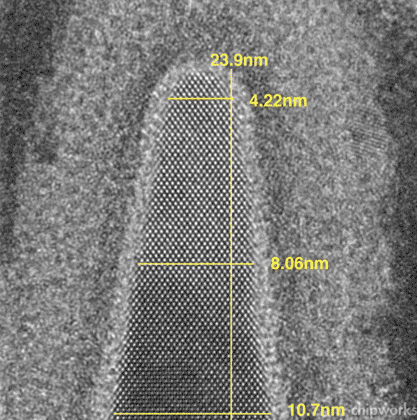
\includegraphics[width=0.3\textwidth]{q_moores_law/tem_silicon_image.png}
			\caption{TEM Image of Intel FINFET Transistor}
			\vspace{-5mm}}
		\label{fig:TEM}
	\end{figure}
\end{enumerate}

	How many atoms across is the feature where it is $4.22 \si{\nano\meter}$ wide?
	\sol{There are 12 atoms (white dots) across the feature.}
	
	\qitem If the most recent 10 \si{\nano\meter} technology was released in 2017, by applying Moore's Law, when would we expect features that are 1 silicon atom wide? Assume that the feature size is reduced by half every time the number of transistors doubles.
	
	\sol{We can write out the equation for the number of transistors on a chip in year $y_n$ relative to previous year $y_0$ as 
		\begin{equation}
		N_{y_n} = N_{y_0}*2^{(y_n-y_0)/t_{double}},
		\end{equation}
		
	where $t_{double}$ is the number of years it takes for the number of transistors to double.
	
	If the feature width $W$ is halved every time the number of transistors doubles, then we can write the equation for the width in future year $y_n$ as 
	\begin{equation}
	W_{y_n} = \frac{W_{y_0}}{2^{(y_n-y_0)/t_{double}}}.
	\end{equation}
	
	Plugging in for $W_{y_0} = 10nm$, $y_0 = 2017$, and $W_{y_n} = 0.543 nm$, and rearranging, we get:
	\begin{equation}
	2^{(y_n-y_0)/t_{double}}= \frac{W_{y_0}}{W_{y_n}}
	\end{equation}
		
	\begin{equation}
	2^{(y_n-2017)/t_{double}}= \frac{10nm}{0.543nm} = 18.4162
	\end{equation}
	
	\begin{equation}
	\frac{y_n-2017}{t_{double}}\text{log}(2)= \text{log}(18.4162)
	\end{equation}
	
	\begin{equation}
	\frac{y_n-2017}{t_{double}}= \text{log}(18.4162)/\text{log}(2) = 4.2029
	\end{equation}
	
	\begin{equation}
	y_n= 4.2029*t_{double}+2017
	\end{equation}
	
	If $t_{double}=1.5$, $y_n = 2023$ and if $t_{double}=2$, $y_n = 2025$. It will take between 6-8 years to reach a feature that is only 1 silicon atom wide if we halve the transistor feature width every 1.5-2 years.
	
	}
	 
	\qitem Do you think Moore's Law can continue forever? Why or why not?
	
	\sol{ No, Moore's Law cannot continue forever. Among other reasons, we cannot create a reliable process that consistently creates features that are 1 atom wide. Also, our use of the materials assumes that the features have some thickness, and that assumption breaks down when there are such few atoms across a device.
	}
	
	
\qns{Controllability Practice}

Consider the system 
\[\vec{x}(t + 1) = 
\begin{bmatrix}
    0 & 1 & -2 \\
    0 & 2 & 0 \\
    -1 & 1 & 0
\end{bmatrix} \vec{x}(t) + 
\begin{bmatrix}
    2 \\ 0 \\ 0
\end{bmatrix} u(t)\]

\begin{enumerate}
    \qitem What is the controllability matrix, $\mathcal{C}$, for this system? What is its column space?

    \sol{
        For a 3-dimensional system,
        \[\mathcal{C} = 
        \begin{bmatrix}
            \vec{b} & A\vec{b} & A^2 \vec{b}
        \end{bmatrix}\]
        Plugging in this system's $A$ and $\vec{b}$, we have
        \[\mathcal{C} = 
        \begin{bmatrix}
            2 & 0 & 4 \\
            0 & 0 & 0 \\
            0 & -2 & 0
        \end{bmatrix}\]
        The column space of $\mathcal{C}$ is the span of its column vectors. 
        The third column is linearily dependendent, so $\text{col}(\mathcal{C})$ is equivalent to the span of its first two columns.
        \[\text{col}(\mathcal{C}) = \text{span}\{ \begin{bmatrix} 1 \\ 0 \\ 0 \end{bmatrix}, \begin{bmatrix} 0 \\ 0 \\ 1 \end{bmatrix}\}\]
    }

    \qitem What is the rank of the controllability matrix? Is the system controllable?

    \sol{
        The controllability matrix has rank 2, so this system is not controllable.
    }

    \qitem Starting at $\vec{x}(0) = \begin{bmatrix} 1 \\ 0 \\ 0 \end{bmatrix}$, what possible states can we reach after one timestep? 
    Two timesteps? Three?

    \sol{
        For one timestep,
        \[\vec{x}(1) = 
        \begin{bmatrix}
            0 & 1 & -2 \\
            0 & 2 & 0 \\
            -1 & 1 & 0
        \end{bmatrix} 
        \begin{bmatrix} 
            1 \\ 0 \\ 0 
        \end{bmatrix}
        + \begin{bmatrix}
            2 \\ 0 \\ 0
        \end{bmatrix} u(0)\]

        Simplifying, we get
        \[\vec{x}(1) =
        \begin{bmatrix} 
            0 \\ 0 \\ -1 
        \end{bmatrix} + 
        \begin{bmatrix} 
            2u(0) \\ 0 \\ 0 
        \end{bmatrix} = 
        \begin{bmatrix} 
            2u(0) \\ 0 \\ -1 
        \end{bmatrix}\]

        Setting $u(0)$ arbitrarily, we can reach any state of the form $\begin{bmatrix} c_1 \\ 0 \\ -1\end{bmatrix}$. \\
        \newline
        For two timesteps,
        \[vec{x}(2) = 
        \begin{bmatrix}
            0 & 1 & -2 \\
            0 & 2 & 0 \\
            -1 & 1 & 0
        \end{bmatrix} 
        \begin{bmatrix} 
            2u(0) \\ 0 \\ -1
        \end{bmatrix}
        + \begin{bmatrix}
            2 \\ 0 \\ 0
        \end{bmatrix} u(1) = 
        \begin{bmatrix} 
            2 + 2u(1) \\ 0 \\ -2u(0)
        \end{bmatrix}\]
        With arbitrary $u(0)$ and $u(1)$, we can reach any state of the form $\begin{bmatrix} c_1 \\ 0 \\ c_2 \end{bmatrix}$. \\
        \newline
        For 3 timesteps,
        \[vec{x}(3) = 
        \begin{bmatrix}
            0 & 1 & -2 \\
            0 & 2 & 0 \\
            -1 & 1 & 0
        \end{bmatrix} 
        \begin{bmatrix} 
            2 + 2u(1) \\ 0 \\ -2u(0)
        \end{bmatrix}
        + \begin{bmatrix}
            2 \\ 0 \\ 0
        \end{bmatrix} u(2) = 
        \begin{bmatrix} 
            4u(0) + 2u(2) \\ 0 \\ -2 - 2u(0)
        \end{bmatrix}\]
        As with 2 timesteps, we can reach any state of the form $\begin{bmatrix} c_1 \\ 0 \\ c_2 \end{bmatrix}$.
    }

    \qitem What is the minimum number of timesteps it takes to reach $\begin{bmatrix} 1 \\ 0 \\ 2 \end{bmatrix}$? 
    What about $\begin{bmatrix} 1 \\ 1 \\ 1 \end{bmatrix}$?

    \sol{
        It takes two timesteps to reach $\begin{bmatrix} 1 \\ 0 \\ 2 \end{bmatrix}$. \\
        $\begin{bmatrix} 1 \\ 0 \\ 2 \end{bmatrix}$ is in the form $\begin{bmatrix} c_1 \\ 0 \\ c_2 \end{bmatrix}$, but not in the form $\begin{bmatrix} c_1 \\ 0 \\ -1 \end{bmatrix}$, so it can be reached in at least two timesteps. \\
        \newline
        It is impossible to reach $\begin{bmatrix} 1 \\ 1 \\ 1 \end{bmatrix}$ in any amount of timesteps.
        The system is not controllable, and we can only reach states of the form $\begin{bmatrix} c_1 \\ 0 \\ c_2 \end{bmatrix}$.
    }
\end{enumerate}

Now answer the same questions for the following system. What differences do you notice?
\[\vec{x}(t + 1) = 
\begin{bmatrix}
    0 & 1 & 0 \\
    0 & 2 & -2 \\
    -1 & 1 & 0
\end{bmatrix} \vec{x}(t) + 
\begin{bmatrix}
    2 \\ 0 \\ 0
\end{bmatrix} u(t)\]

\sol {
    \begin{enumerate}
        \qitem  
        \[\mathcal{C} = 
        \begin{bmatrix}
            \vec{b} & A\vec{b} & A^2 \vec{b}
        \end{bmatrix} = 
        \begin{bmatrix}
            2 & 0 & 0 \\
            0 & 0 & 4 \\
            0 & -2 & 0
        \end{bmatrix}\]
        The column space of this matrix spans $\mathbb{R}^3$.

        \qitem The controllability matrix has rank 3, so the system is controllable.

        \qitem 
        For one timestep, 
        \[\vec{x}(1) = 
        \begin{bmatrix}
            0 & 1 & 0 \\
            0 & 2 & -2 \\
            -1 & 1 & 0
        \end{bmatrix} 
        \begin{bmatrix} 
            1 \\ 0 \\ 0 
        \end{bmatrix}
        + \begin{bmatrix}
            2 \\ 0 \\ 0
        \end{bmatrix} u(0) =
        \begin{bmatrix} 
            2u(0) \\ 0 \\ -1 
        \end{bmatrix}\]
        So, we can reach any state of the form $\begin{bmatrix} c_1 \\ 0 \\ -1 \end{bmatrix}$. \\
        \newline

        For two timesteps,
        \[\vec{x}(2) = 
        \begin{bmatrix}
            0 & 1 & 0 \\
            0 & 2 & -2 \\
            -1 & 1 & 0
        \end{bmatrix} 
        \begin{bmatrix} 
            2u(0) \\ 0 \\ -1 
        \end{bmatrix}
        + \begin{bmatrix}
            2 \\ 0 \\ 0
        \end{bmatrix} u(1) =
        \begin{bmatrix} 
            2u(1) \\ 2 \\ -2u(0) 
        \end{bmatrix}\]
        We can reach any state of the form $\begin{bmatrix} c_1 \\ 2 \\ c_2 \end{bmatrix}$. \\
        \newline

        For three timesteps,
        \[\vec{x}(3) = 
        \begin{bmatrix}
            0 & 1 & 0 \\
            0 & 2 & -2 \\
            -1 & 1 & 0
        \end{bmatrix} 
        \begin{bmatrix} 
            2u(1) \\ 2 \\ -2u(0) 
        \end{bmatrix}
        + \begin{bmatrix}
            2 \\ 0 \\ 0
        \end{bmatrix} u(2) =
        \begin{bmatrix} 
            2 + 2u(2) \\ 4 + 4u(0) \\ 2 - 2u(1) 
        \end{bmatrix}\] 
        We can reach any state in $\mathbb{R}^3$ in three timesteps.

        \qitem
        The system is controllable, so we can reach any state in three timesteps.
        We cannot reach either state in fewer timesteps because neither $\begin{bmatrix} 1 \\ 0 \\ 2 \end{bmatrix}$ nor $\begin{bmatrix} 1 \\ 1 \\ 1 \end{bmatrix}$ are in the form $\begin{bmatrix} c_1 \\ 0 \\ -1 \end{bmatrix}$ or $\begin{bmatrix} c_1 \\ 2 \\ c_2 \end{bmatrix}$.
    
    \end{enumerate}
}		

\end{qunlist}

\end{document}
